\newpage\section{An{á}lisis sensor Aceler{ó}metro}

En este apartado abordaremos el análisis del sensor acelerómetro que es ampliamente utilizado para detectar cuando una persona sufre una caída; de acuerdo a la investigación se deberán responder las siguientes preguntas: ¿cómo determinamos qué una persona está cayendo?, ¿cuáles son los rangos en los que se establece que una persona sufrió una caída?, ¿cuáles son los motivos por los que se seleccionó el acelerómetro \textbf{MPU-6050}? y por último, ¿cuál es el funcionamiento y las características principales del acelerómetro \textbf{MPU-6050}?. \\

\subsection{Etapas de una caída}

Una caída comprende 4 etapas, en las cuales se observa una aceleración diferente y las etapas críticas tienden a ser los rangos de evaluación para definir si se sufrió o no dicha acción. A continuación, se describen dichas etapas \cite{cuarentaynueve}:

\begin{figure}[h]
	\centering
	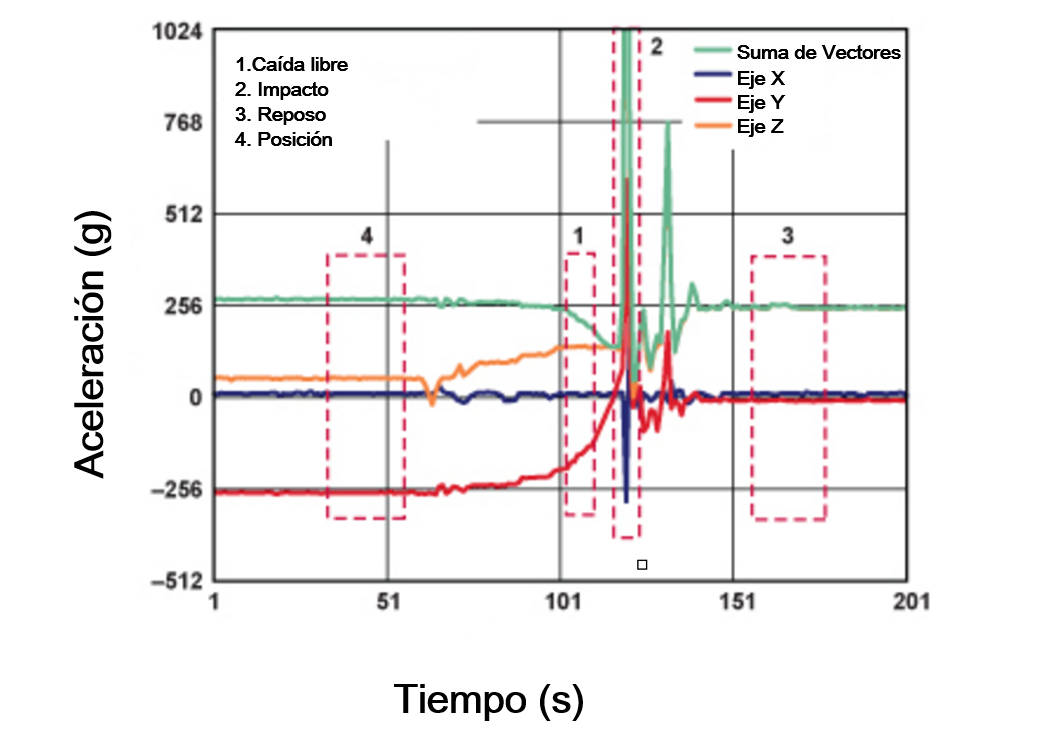
\includegraphics[scale=0.35]{analisis/imagenes/etapas_caida}
	\textbf{\caption{\small{Gráfica 2.1 Puntos de interés en la señal que muestra: (a) posturas al sufrir una caída y (b) actividades cotidianas \cite{cuarentaynueve}.}}}
	\label{fig:sensorcaida}
\end{figure}

\begin{itemize}
	\item \textbf{Caída libre}: Cuando una persona pierde el equilibrio se dirige hacia el suelo con un movimiento de caída libre y es justo donde se da el primer cambio en la señal; en esta etapa se contempla el fenómeno de gravedad y la suma vectorial de la aceleración se reflejará menor que 1g y mayor que $0g (1g > a > g)$. 
	\item \textbf{Impacto}: El cuerpo tendrá un choque con el suelo, pared u objeto, en esta etapa la señal tendrá un cambio significativo teniendo un pico muy elevado con valores en la aceleración de entre $2g y 12g$.
	\item \textbf{Reposo}: El cuerpo humano, después de caer y hacer impacto, no puede levantarse de inmediato; por lo que permanece en una posición inmóvil durante un período de tiempo (este puede ser corto o largo dependiendo de la gravedad de la caída).
	\item \textbf{Posición final}: Después de una caída, el cuerpo de la persona estará en una orientación diferente a la anterior, por lo que la aceleración estática en tres ejes será diferente de la situación inicial antes de la caída. Se hace un muestreo de la aceleración antes (muestreo inicial) y después (muestreo final) de la caída, se comparan los datos de muestreo y se evalúa; si la diferencia entre los datos de muestreo y supera un umbral de $0,7 g$ se declara como caída.
\end{itemize}

\subsection{Algoritmo basado en umbrales y orientación}

Simplemente se basa en detectar las cuatro etapas de las caídas: caída libre, impacto, reposo y posición final.	Se describirá el siguiente algoritmo el cual se abordará en este proyecto para detectar las caídas.

\begin{figure}[h]
	\centering
	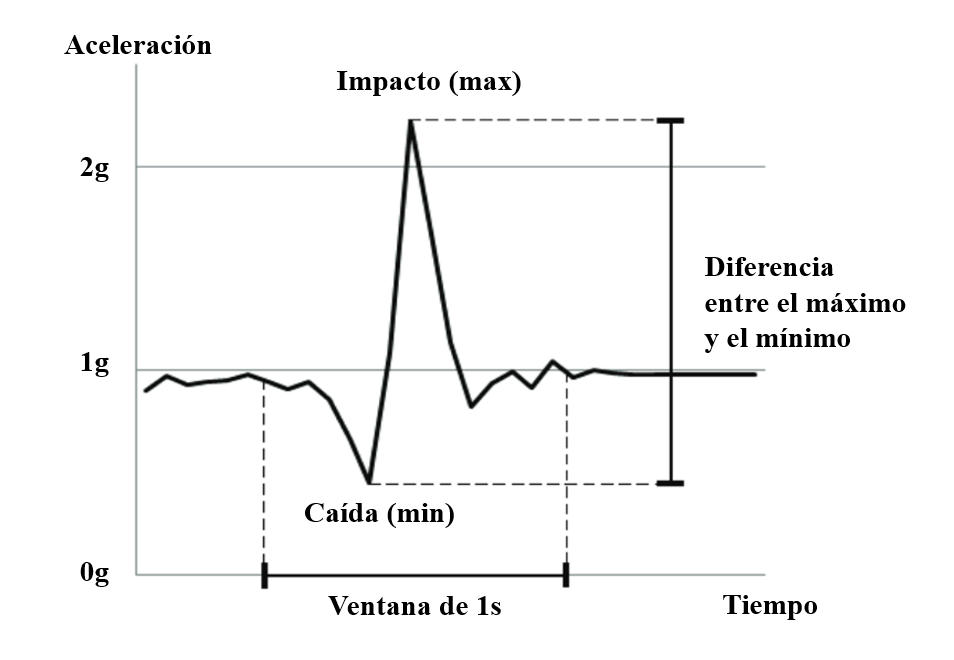
\includegraphics[scale=0.35]{analisis/imagenes/aceleracion}
	\textbf{\caption{\small{Gráfica 2.2 Patrón de la aceleración durante una caída \cite{cincuenta}.}}}
	\label{fig:sensorcaida2}
\end{figure}

\begin{enumerate}
	\item Un acelerómetro registra que una persona en reposo tiene de $1g$ (gravedad de la Tierra) de aceleración y durante la caída libre dicha aceleración tiende a 0 g. Cuando una persona comienza a caer, la aceleración disminuye de $1g \quad a \quad 0.5g$ aproximadamente (nunca se logra caída libre perfecta). 
	\item Tras el impacto con el suelo, se mide un alto y bajo aumento en la aceleración, lo cual nos da un pico muy largo.
	\item En el umbral, se utiliza la longitud del vector de aceleración, ignorando la dirección de la aceleración. En el lapso de un segundo se mide la aceleración máxima y mínima, si la diferencia entre estas aceleraciones: máxima y mínima es mayor de 1g y la máxima se produce después de la mínima, se declara que se ha producido una caída. 
	\item Sea $z$ el eje apuntando hacia abajo cuando la persona está de pie en posición vertical. El ángulo entre el vector de aceleración y el eje $z$, indica la orientación de la persona, y se calcula mediante la siguiente fórmula: 
\end{enumerate}

\begin{equation}
cos\phi \equiv \frac{{\alpha}_{z}}{{\alpha}_{x^2}+{\alpha}_{y^2}+{\alpha}_{z^2}}
\end{equation}

Puesto que cada persona tiene su postura característica y el acelerómetro puede no siempre ser usado exactamente de la misma manera, la orientación promedio de cada persona durante 15 segundos de caminar se mide como ${\phi}_{0}$. Posteriormente, cuando se mide una nueva orientación $\phi$, se normaliza como sigue: ${\phi}_{norm} = \phi – {\phi}_{0}$. Una persona es considerada orientada hacia arriba, si $-30^{\circ} < {\phi}_{norm} < 30^{\circ}$. Por lo cual, si se ha detectado una aceleración que supera el umbral como se ha descrito anteriormente, y la orientación de la persona durante 10 segundos no es en posición vertical, se declara que se ha producido una caída \cite{cincuenta}.

\subsection{Selección y tabla comparativa de acelerómetros}

El acelerómetro seleccionado fue el MPU-6050, de acuerdo a la investigación en la tabla comparativa, esto fue porque incluye un giroscopio, su tipo de interfaz es digital I$^{2}$C, el costo es promedio comparado con los demás, además de tener un diseño para el bajo consumo de energía, de estas características podemos resaltar que es ampliamente usado en: teléfonos inteligentes, tabletas y sensores portátiles. \\

\begin{table}[htb]
	\centering
	\begin{tabular}{|p{1cm}|p{5cm}|p{2.5cm}|p{2.5cm}|p{2.5cm}}
		\hline
		\multicolumn{5}{|c|}{Tabla comparativa de acelerómetros} \\
		\cline{1-5} \hline
		Modelo & MPU-6050 & ADXL345 & MMA8451Q & LIS331HH \\
		\hline 
		Fabricante & Inven Sense & Analog Devices & Freescale & STMicroelectronics \\ \cline{1-5}
		\hline 
		Salida & Digital 8 bits & Digital de 12 bits & Digital 13 bits & Digital 16 bits \\ \cline{1-5}
		\hline
		Interfaz de comunicación & I2C & SPI, I2C & I2C & I2C \\ \cline{1-5}
		\hline
		Rango de medición & ±2g, ±4g, ±8g, ±16g & ±16 & +/- 8g & +/- 24g \\ \cline{1-5}
		\hline
		Dimensión & 4mm x 4mm x 0.9mm & 3mm x 5mm x 1mm & 3mm x 5mm x 1mm & 3mm x 5mm x 1mm \\ \cline{1-5}
		\hline
		Ejes & 3 & 3 & 3 & 3 \\ \cline{1-5}
		\hline
		Precisión & 1mg/LSB & 4 mg/LSB & 0.98 g/LSB & 3 mg/LSB (a +/-12g) \\ \cline{1-5}
		\hline
		Alimentación & 2.375V a 3.46V & 2V a 3.6V & 1.95V a 3.6V & 2.16V a 3.6V \\ \cline{1-5} 
		\hline
		Corriente Máxima & & 40uA & 165uA & 10uA \\ \cline{1-5} 
		\hline
		Características adicionales & Incluye giroscopio & & & \\ \cline{1-5} 
		\hline
		Frecuencia de muestreo & Hasta 400kHz & Hasta 3200 Hz & Hasta 800 Hz & Hasta 1 KHz \\ \cline{1-5} 
		\hline
		Rango de temperatura & -40$^\circ$C a +85$^\circ$C & -40$^\circ$C a +85$^\circ$C & -40$^\circ$C a +85$^\circ$C & -40$^\circ$C a +85$^\circ$C \\ \cline{1-5} 
		\hline
		Calibración & Programable & De Fábrica & De Fábrica & De Fábrica \\ \cline{1-5} 
		\hline
		Montaje superficial & si & si & si & si \\ \cline{1-5} 
		\hline
		Costo & \$3.99 & \$6.93 & \$2.16 & \$5.97 \\ \cline{1-5} 
		\hline
	\end{tabular}
	\textbf{\caption{\small{\textbf{Escenarios y posturas en los que el acelerómetro realizará muestreo.}}}}
\end{table}

\subsection{Características, especificaciones y funcionamiento interno del acelerómetro MPU-6050}

El acelerómetro MPU-6050 cuenta con un acelerómetro y un giroscopio internos, este dispositivo es altamente usado en aplicaciones basadas en video, estabilización de imágenes, seguridad en autenticación, reconocimiento de gestos, control de movimiento, sensores para la salud, sensores para condición física, sensores para deporte y juguetes. En el siguiente apartado se mostrarán las características, diagrama a bloques y la descripción con las que cuenta dicho dispositivo.

\begin{itemize}
	\item \textbf{Características}
\end{itemize}

En la tabla 2.XXXIV se marcarán las características principales para el dispositivo. \\

\begin{table}[htb]
	\begin{tabular}{|p{1.8cm}|p{1.8cm}|p{1.3cm}|p{1.8cm}|p{2.3cm}|p{1.3cm}|}
		\hline 
		Sensor & Tiempo de Respuesta & Salida & Resolución & Campo de medición & Precio \\ 
		\hline 
		Amphenol MA100 & En el aire 15s \par En agua 2.0s & Resistiva & 1$^{\circ}$C & 0$^{\circ}$C a 50$^{\circ}$C  & \$8.00 \\ 
		\hline 
		Amphenol MA200 & En el aire 35s \par En agua 0.6s & Resistiva & 1$^{\circ}$C & 0$^{\circ}$C a 50$^{\circ}$C  & \$8.00 \\ 
		\hline 
		Amphenol MA300 & En el aire 45s \par En agua 2s & Resistiva & 1$^{\circ}$C & 0$^{\circ}$C a 50$^{\circ}$C  & \$8.00 \\  
		\hline 
		LM334 & --- & Corriente & 1.04$^{\circ}$C & 0$^{\circ}$C a 70$^{\circ}$C & \$47.5 \\ 
		\hline 
		LM35 & 1s & Voltaje & 10mv/$^{\circ}$C & -55$^{\circ}$C a 150$^{\circ}$C & \$42.00 \\ 
		\hline 
		MLX90614 & 5ms & Voltaje & 0.2$^{\circ}$C & -70$^{\circ}$C a 380$^{\circ}$C & \$280.00 \\ 
		\hline 
	\end{tabular} 
\textbf{\caption{\small{\textbf{Características de sensores de temperatura.}}}}
\end{table}


Analizando las propiedades eléctricas de los sensores elegimos el sensor MLX90614 por su sensibilidad de 0.2$^{\circ}$C ya que para nuestro proyecto es necesario medir con una sensibilidad menor a 1$^{\circ}$C, debido a que las vulnerabilidades se presentan al tener temperaturas que pasan en $\pm$0.2$^{\circ}$C el rango aceptable (36.5$^{\circ}$C a 37.2$^{\circ}$C), otra característica que nos es importante es el tiempo de respuesta del sensor que es en el orden de los milisegundos, la comunicación es otro aspecto que se consideró, para poder comunicarlo con el microcontrolador, en este caso es $I^2 C$, y por ultimo tenemos un precio aceptable y una alimentación estándar de 3v a 5v.

\subsection{Sensor MLX90614}


En este aparto explicaremos el funcionamiento del sensor de temperatura MLX90614 indicando el funcionamiento interno para medir la temperatura. \\

El sensor de temperatura MLX90614 es un sensor de temperatura infrarrojo, el cual capta la temperatura promedio de un lector infrarrojo que mide la energía desprendida por los objetos. Esté sensor infrarrojo tiene una conexión en serie de dos termopares, una se encuentra dentro soporte del chip conectada con un sensor que mide la temperatura del chip, y la otra está colocada en una membrana delgada que está unida con el lector infrarrojo esté absorbe la radiación de la membrana, ya sea caliente o fría \cite{cuarentaycinco}.

\begin{figure}[h]
	\centering
	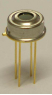
\includegraphics{analisis/imagenes/sensor_temperatura}
	\textbf{\caption{\small{Sensor de temperatura MLX9614 \cite{cuarentaycinco}.}}}
	\label{fig:sensortemperatura}
\end{figure}

A continuación, explicaremos que es un termopar y cómo es que funciona, para poder entender cómo es que funciona en sensor MLX90614.
Un termopar es una unión de dos metales distintos unidos en un extremo, cuando a la unión se le presenta una temperatura distinta a la temperatura de la unión se genera un voltaje muy pequeño (efecto Seebeck) del orden de los milivolts, esté aumenta conforme la temperatura se incrementa (no es lineal), dependiendo del tipo de termopar existe una relación temperatura-voltaje. \\

Son utilizadas como sensores de temperatura, el principal inconveniente es la necesidad de compensar a cero, esto se debe a que, al tomar las lecturas en el otro extremo del termopar, se une con otro metal distinto (creando otro termopar) produciendo otro voltaje, el cual es proporcional a la temperatura del ambiente por lo que es necesario medir la temperatura en la unión donde se realiza la lectura, utilizando un sensor que obtenga la temperatura del ambiente. Las dos temperaturas de suman para crear la compensación y así obtener la temperatura real. \\

En la figura 2.4 se muestra los puntos de intersección entre los metales, los puntos en los que se obtiene diferentes temperaturas, siendo T la temperatura del objeto y Ta la temperatura del ambiente.

\begin{figure}
	\centering
	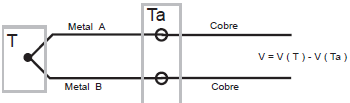
\includegraphics{analisis/imagenes/esquema_termopar}
	\textbf{\caption{\small{Esquema de un termopar (V es el voltaje total obtenido por un volmetro) \cite{cuarentayseis}.}}}
	\label{fig:esquematermopar}
\end{figure}

V(Ta) es el voltaje obtenido por la unión del metal A y el cobre \\

De tal forma que se tienen tres uniones la unión del metal A y metal B, la unión del cobre con el metal B y la unión del metal A con el cobre. Teniendo la siguiente ecuación. \\

\begin{equation}
	V_{Total} \quad = \quad V_{AB(T)} \quad - \quad V_{CuA(Ta) \quad - \quad V_{CuB(Ta)}}
\end{equation}

\begin{equation}
	V_{Total} \quad = \quad V_{AB(T)} \quad - \quad[V_{CuA(Ta) \quad - \quad V_{CuB(Ta)}}]
\end{equation}

\begin{equation}
	V_{Total} \quad = \quad V_{AB(T)} \quad - \quad V_{AB(Ta)}
\end{equation}

\begin{equation}
V_{AB(T)} \quad = \quad V_{Total} \quad - \quad V_{AB(Ta)}
\end{equation}

Posteriormente una vez que se tiene esta ecuación se busca en la tabla del termopar el voltaje $V_{AB(Ta)}$ de acuerdo a la temperatura ambiente, obteniendo el voltaje $V_{AB(T)}$ se puede saber la temperatura de la unión AB, buscando en la tabla del termopar AB, que temperatura corresponde al voltaje $V_{AB(T)}$. \\

Una vez explicado el funcionamiento de un termopar podremos entender ¿Cómo es que mide la temperatura el sensor MLX90614? El sensor MLX90614 tiene internamente dos sensores para medir la temperatura, estos sensores están conectados por medio de un termopar, la primera unión es con el sensor infrarrojo (la membrana) y la segunda con un sensor que mide la temperatura del ambiente, para posteriormente calcular la compensación del termopar y calcular la temperatura del infrarrojo \cite{cuarentayseis}. \\

La señal emitida por el termopar responde a la siguiente ecuación:

\begin{equation}
V_{Ir(Ta,To)} \quad = \quad A \quad \ast \quad (To^4 \quad - \quad Ta^4)
\end{equation}

Donde: \\

\begin{itemize}
	\item $V_{Ir(Ta,To)}$ es el voltaje de respuesta del termopar.
	\item $A$ es la sensibilidad total del infrarrojo.
	\item $To$ es la temperatura obtenida por el infrarrojo.
	\item $Ta$ es la temperatura del ambiente.
\end{itemize}

El principio de los sensores infrarrojos es la radiación infrarroja, está es la parte de la luz solar que se descompone al reflejar la luz solar a través de un prisma, la cual pose energía, teniendo relación con el espectro electromagnético. \\

La energía desprendida por la radiación del campo electromagnético se puede medir mediante una relación con las curvas emitidas por un cuerpo oscuro o negro (emisividad), mientras que los objetos con una temperatura por encima del cero absoluto irradian energía \cite{cuarentaysiete}.

\begin{figure}
	\centering
	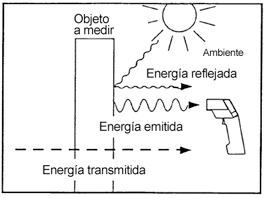
\includegraphics{analisis/imagenes/factor}
	\textbf{\caption{\small{Factor de emisión \cite{cuarentaysiete}.}}}
	\label{fig:factor}
\end{figure}

La cantidad de energía crece de manera proporcional a la cuarta potencia de la temperatura, es por ello que en la ecuación 2.20 las temperaturas $(To^4 \quad - \quad Ta^4)$, en cuanto a A es un factor de emisión que se obtuvo de la relación de las radiaciones que emite un cuerpo gris y un cuerpo negro a igual que la temperatura, estos cuerpos tienen el mismo factor de emisión  en todas las longitudes de onda, por el contrario un cuerpo diferente del gris y el negro cambia su factor de emisión con respecto a la longitud de onda. \\

La temperatura del sensor es necesaria para medir la temperatura del chip, una vez que mide la temperatura del objeto y el ambiente, se calcula la temperatura del chip, los cálculos se realizan por el DPS (Procesador de señal digital) produciendo salidas digitales lineales proporcionales a las temperaturas medidas. \\

Temperatura ambiente \\

El sensor calcula la temperatura mediante termopares y sensores de temperatura internos, todas las condiciones de los sensores y los datos procesados se manejan dentro del chip, mientras que las lecturas de la temperatura del sensor se encuentran en la memoria de acceso aleatorio (RAM) \cite{cuarentaycinco}. \\

La resolución de la temperatura calculada es de 0.02$^{\circ}$C debido a que el convertidor analógico digital (ADC) es de 17 bits, cada bit representa 0.02$^{\circ}$C, el sensor esta calibrado de fábrica con un rango de -40$^{\circ}$C a +125$^{\circ}$C, el valor digital de la temperatura ambiente se encuentra en la RAM en la celda 0x06. \\

Los valores de las temperaturas se encuentran en un formato hexadecimal, la fórmula para obtener la temperatura ambiente en grados $^{\circ}$K es la siguiente:

\begin{equation}
	Ta \quad = \quad {(Valor \quad del \quad registro \quad 0\times06)}_{10} \quad \ast \quad 0\ldotp02
\end{equation}

\begin{itemize}
	\item $Ta$ es el valor de la temperatura ambiente en grados Kelvin.
	\item Es el valor del registro después de convertir de hexadecimal a decimal.
	\item 0.02 es el valor de cada bit.
\end{itemize}

Ejemplos: \\

Tenemos que el valor de la temperatura es 0x2DE4 y se desea saber la temperatura en grados Kelvin como Celsius. \\

\begin{itemize}
	\item El primer pasó el convertir de hexadecimal a decimal el valor del registro.
\end{itemize}

Para convertir de hexadecimal a decimal se utiliza la base 16 y la base 10, multiplicamos cada dígito con el valor de la potencia base dieciséis que le corresponde, siendo el menos significativo el dígito de la derecha. \\

\begin{equation}
Valor \quad digital \quad = \quad 4\ast16^0 \quad + \quad 14\ast16^1 \quad + \quad 13\ast16^2 \quad + \quad 2\ast16^2 
\end{equation}

\begin{equation}
Valor \quad digital \quad = \quad 4 \quad + \quad 224 \quad + \quad 3328 \quad + \quad 8192 
\end{equation}

\begin{equation}
Valor \quad digital \quad = \quad {11748}_{10}  
\end{equation}

El segundo paso es multiplicar la resolución obtenida por el valor digital, obteniendo la temperatura en grados Kelvin, para pasarlos a Celsius se resta 273. \\

\begin{equation}
Ta \quad = \quad 11748 \quad \ast \quad 0\ldotp02
\end{equation}

\begin{equation}
Ta \quad = \quad 234\ldotp96^{\circ}K
\end{equation}

\begin{equation}
Ta \quad = \quad 234\ldotp96 \quad - \quad 273
\end{equation}

\begin{equation}
Ta \quad = \quad - 38\ldotp04^{\circ}C
\end{equation}

El valor mínimo de medición de la temperatura del ambiente es -38.2$^{\circ}$C y el valor máximo medido es 125$^{\circ}$C. \\
 
Temperatura Objeto \\

La temperatura del objeto se encuentra en la celda 0x07, se calcula de la misma manera que la del ambiente, el bit más significativo indica un error, al medir una temperatura que sobre pase los 382.19$^{\circ}$C o en su valor hexadecimal 0x7FFF. \\

Para obtener las mediciones de temperatura, el sensor realiza cálculos, y el resultado lo obtiene lineal, estos pasos se realizan en el núcleo del sensor (en el chip), se ejecuta un programa de la memoria de solo lectura (ROM) antes de encender o de resetear, el chip inicia con los datos de calibración, durante esta fase se selecciona el número de sensor infrarrojo que se utilizará y se decide el rango de temperatura que tendrá en sensor, las rutinas de medición, compensación y la muestra de la  temperatura lineal se corren dentro del término bucle \cite{cuarentaycinco}. \\

El sensor de temperatura utiliza los siguientes filtros para acondicionar las lecturas de temperatura: \\

Filtro Pasa-banda \\

Un filtro pasa-banda permite pasar las frecuencias que están situadas en una determinada banda de frecuencia, es decir entre dos determinadas frecuencias y rechaza las frecuencias fuera de esa banda. \\

Filtros digitales \\

Un filtro digital se puede definir como un proceso computacional o algoritmo mediante el cual una señal digital es transformada en una segunda secuencia de muestras. \\

Respuesta impulsional \\

Es la relación de un filtro a un impulso que se envía a su entrada, la respuesta impulsional caracteriza   a un filtro en el dominio temporal. El funcionamiento de un filtro digital consiste en sumar una señal de entrada a su salida o viceversa. \\

Filtros digital IR y IIR \\

El filtro IR (Respuesta impulsional finita) retarda ligeramente una copia de la señal de entrada (uno o varios periodos) y la suma a la señal de respuesta del filtro \cite{cuarentayocho}. \\ 

\begin{figure}[h]
	\centering
	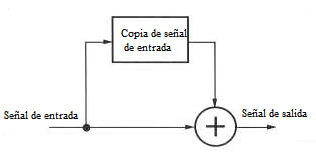
\includegraphics{analisis/imagenes/principio_filtro}
	\textbf{\caption{\small{Principio filtro FIR \cite{cuarentayocho}.}}}
	\label{fig:principiofiltro}
\end{figure}

El filtro digital IIR (Respuesta impulsional infinita) procesa una señal de entrada, la señal obtenida se combina con la de entrada.

\begin{figure}
	\centering
	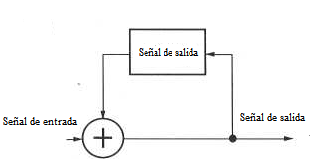
\includegraphics{analisis/imagenes/filtro_iir}
	\textbf{\caption{\small{Principio filtro IIR \cite{cuarentayocho}.}}}
	\label{fig:filtroiir}
\end{figure}

Los filtros se pueden describir mediante ecuaciones que relacionan la señal de entrada con una señal de salida en el domino digital. De manera que la salida del filtro se especifica como un resultado de sumas, restas y multiplicaciones de muestras de entradas actuales y anteriores. \\

Ecuación de los filtros digitales FIR \\

Se puede definir como la combinación lineal de muestras de la entrada presente o pasadas, se expresa de la siguiente forma:

\begin{equation}
	y[n] \quad = \quad a0 \cdot x[n] \quad + \quad a1 \cdot x[n - 1] \quad + \quad a2 \cdot x[n - 2] \quad + \ldots + \quad aN \cdot x[n - N]
\end{equation}

Esta ecuación expresa que la muestra actual de la salida $y[n]$ es igual a la suma de las muestras de la entrada actual $x[n]$ multiplicada por el factor $a0$ y de la muestra anterior $x[n – 1]$ multiplicando por el factor $a1$, y de todas las muestras anteriores hasta el instante $[n - N]$ multiplicado por su correspondiente factor. Donde los factores modifican las características de la señal \cite{cuarentayocho}. \\

Señal digital: \\

\begin{equation}
	x \quad = \quad \{1,0,0,0,0,0,0,\ldots\}
\end{equation}

Señal de salida: \\

\begin{equation}
x \quad = \quad \{a0,a1,a2,a3,\ldots,aN,0,0,0,\ldots\}
\end{equation}

Ecuación de filtro digital IIR \\

Los filtros IIR se distinguen de los filtros FIR por la presencia de una recursividad, la señal de salida del filtro retroalimenta el filtro, esté método permite implementar filtros con respuesta más compleja y con menos datos, al retroalimentar la entrada la respuesta impulsional tiene una duración potencial infinita. \\

\begin{equation*}
	\begin{split}
	y[n] \quad = \quad a0 \cdot x[n] \quad + \quad a1 \cdot x[n - 1] \quad + \quad a2 \cdot x[n - 2] \quad + \ldots + \quad \\ aN \cdot x[n - N] \quad + \quad - \quad b1 \cdot y[n-1] \quad - \quad b2 \cdot y[n-2] \quad - \quad \\ b3 \cdot y[n-3]  \quad \ldots \quad - \quad bM \cdot y[n-M]
	\end{split}		
\end{equation*}

Esta ecuación expresa que la salida es función de N+1 muestras de la entrada (actuales y N anteriores), así como de M muestras anteriores de salida. \\

Diferencia entre los filtros digitales \\

Los filtros FIR ofrecen en general una respuesta de fase más lineal y no entran jamás en oscilación, pero requieren de un gran número de muestras haciéndolos más caros computacionalmente, mientras que los filtros IIR son muy eficaces y pueden proporcionar pendientes de corte muy pronunciadas, pero tienden a entrar en resonancia\cite{cuarentayocho}. \\

Los procesos que se realizan en el sensor se dividen en 3 partes: \\

Desviación del infrarrojo \\

\begin{itemize}
	\item Se mide la desviación con la FIR, fijando la longitud de la respuesta del filtro.
	\item Agrega al filtrado la IIR fijando su longitud, el resultado es almacenado dentro de la RAM en la variable (registro) $IR_{os}$.
	\item Se obtiene otra medida con FIR del filtro, fijando la longitud de la respuesta.
	\item Compensación de la desviación.
	\item Se agrega un proceso adicional programando la longitud IIR, el resultado se almacena dentro de la RAM en $IR_G$.
	\item Se calcula la compensación obtenida, el resultado se almacena dentro de la RAM en $K_G$.
\end{itemize}

Temperatura del Objeto \\

Estos son los procesos que realizan para obtener la temperatura del objeto, el sensor MLX90614 tiene dos sensores infrarrojos internos. \\

\begin{itemize}
	\item Medición del sensor infrarrojo se programa la longitud FIR del filtro.
	\item Compensación de la desviación.
	\item Gana compensación.
	\item Se filtra, programando la longitud IIR del filtro, se almacena el resultado dentro de la RAM en la dirección 0x04 en $IR1_D$.
	\item El cálculo de la temperatura del objeto, se almacena en la dirección 0x07 en $T_{02}$.
	
\end{itemize}

El mismo procedimiento se realiza con el segundo sensor infrarrojo \cite{cuarentaycinco}.

